\chapter{The Equations of a Star}
\label{ch:structure}

\newcommand{\TwelveXiOne}{3.1416}
\newcommand{\TwelveOmegaOne}{3.1416}
\newcommand{\TwelveRhoRatioOne}{3.29}
\newcommand{\TwelveXiOneHalf}{3.6538}
\newcommand{\TwelveOmegaOneHalf}{2.7141}
\newcommand{\TwelveRhoRatioOneHalf}{5.99}
\newcommand{\TwelveXiThree}{6.8968}
\newcommand{\TwelveOmegaThree}{2.0182}
\newcommand{\TwelveRhoRatioThree}{54.18}
\newcommand{\TwelveIsoRatio}{0.991}
\newcommand{\TwelveSunRhoC}{7.64\times10^{4}}
\newcommand{\TwelveSunPC}{1.25\times10^{16}}
\newcommand{\TwelveSunTC}{1.22\times10^{7}}
\newcommand{\TwelveBetaSun}{0.9995}
\newcommand{\TwelveBetaTen}{0.961}
\newcommand{\TwelveBetaHundred}{0.558}
\newcommand{\TwelveBetaThousand}{0.204}

\newcommand{\TwelveHRN}{20\,298}
\newcommand{\TwelveHRMaxPc}{220}
\newcommand{\TwelveHRNwd}{11\,990}


A star is a ball of gas in hydrostatic equilibrium (Section~\ref{sg:sec:hse}), heated inside by nuclear burning and losing energy from its surface as light (Chapter~\ref{ch:radiation}). Its whole structure, the density, pressure, temperature and luminosity at every depth, follows from four equations. Each equation is one of the principles at work. Three properties of the gas, its pressure, its opacity and its rate of burning, close the four equations, and each of those is again one of the principles.

The same four equations, with their boundary conditions, are what stellar-evolution codes solve. Understanding them is understanding how a star is computed.

% ==============================================================================
\section{The Unknowns}
\label{st:sec:unknowns}

Chapter~\ref{ch:selfgrav} described a star at each radius $r$, with $m(r)$ the mass inside.

Inside a real star the gas does not stay at one radius. As the star contracts or expands, a given parcel of gas moves, and the radius stops being a good label for it. What follows the gas is the mass inside it.

Think of the rings of a tree. As the tree grows, every ring moves outward, but the ring laid down in a given year stays the same ring. Counting rings from the centre labels the wood, whatever the size of the trunk.

Inside a star the mass coordinate $m$ plays the part of the ring count. The shell of gas with mass $m$ inside it keeps that label while the star contracts, expands or burns. Its composition changes only by its own burning, so everything that happens to a parcel happens at fixed $m$. The four equations are therefore written with $m$, from $0$ at the centre to $M$ at the surface, as the independent variable.

In numbers, the Sun's radius has grown by about $10\%$ since it began to burn hydrogen, but the shell holding the inner half of its mass is still the shell with $m=M_\odot/2$.

The picture is a set of nested shells labelled by the mass they enclose, not by their radius.

Fluid dynamics calls this the Lagrangian description, following the fluid, as opposed to the Eulerian description at fixed points of space. It gives four unknown functions of $m$. They are the radius $r(m)$, the pressure $P(m)$, the temperature $T(m)$ and the luminosity $L(m)$ flowing out through the shell.

% ==============================================================================
\section{The Four Equations}
\label{st:sec:four_equations}

Hydrostatic equilibrium (Eq.~\eqref{sg:eq:hse}) and the flow of light (Eq.~\eqref{rad:eq:radiative_transport}) have been derived already.

They are two of the four equations, and both are written with $r$. A complete model needs the other two, how the mass relates to the radius and how the luminosity builds up, and needs all four with $m$ as the variable.

Think of a household budget kept month by month. One line records the money coming in. Another records the money going out. The balance at the end of each month follows from the balance before plus the difference. Nothing else is needed, and nothing can be left out.

A star keeps four such accounts, shell by shell, for space, momentum, energy and the flow of heat. Each one says how a quantity changes from one shell to the next. Mass and energy are conservation (P1). Momentum is conservation with the gravity of a sphere (P1 and P2). The flow of heat is a random walk of light (P5), or, where that is too slow, the bulk motion of the gas itself.

In numbers, the Sun's luminosity of $3.83\times10^{26}\,\mathrm W$ is built up almost entirely in the inner quarter of its radius, where the burning happens, and then carried unchanged through the outer three quarters.

The picture is a stack of shells, with each equation stepping one quantity from a shell to the next.

The same four accounts, with the same structure, describe the interior of a planet (with no burning), the core of a white dwarf (with no burning and degenerate gas) and the envelope of an accreting neutron star. They give the four equations of stellar structure.

\paragraph{Mass.} Inverting the definition of $m(r)$, Eq.~\eqref{pr:eq:mass_inside},
\begin{equation}
	\boxed{\dv{r}{m}=\frac{1}{4\pi r^2\rho}.}
	\label{st:eq:mass}
\end{equation}

\paragraph{Momentum.} Hydrostatic equilibrium \eqref{sg:eq:hse}, divided by $\dv*{m}{r}=4\pi r^2\rho$,
\begin{align}
	\dv{P}{m}
	&\eqby{1} \dv{P}{r}\,\dv{r}{m} \nonumber\\
	&\eqby{2} -\frac{Gm\rho}{r^2}\,\frac{1}{4\pi r^2\rho} \nonumber\\
	&= -\frac{Gm}{4\pi r^4} .
\end{align}
\begin{explain}
	\item The chain rule.
	\item Eq.~\eqref{sg:eq:hse} and Eq.~\eqref{st:eq:mass}.
\end{explain}
\begin{equation}
	\boxed{\dv{P}{m}=-\frac{Gm}{4\pi r^4}.}
	\label{st:eq:momentum}
\end{equation}
The density has dropped out. The pressure falls outward at a rate set by gravity alone.

\paragraph{Energy.} Take the shell between $m$ and $m+dm$. Nuclear burning releases energy in it at the rate $\varepsilon\,dm$, where $\varepsilon$ is the energy released per unit mass and time. Light carries $L(m)$ in through its inner face and $L(m+dm)$ out through its outer face. Whatever is left heats the shell. With $s$ the entropy per unit mass, the heat added to the shell per unit time is $T\,(\dv*{s}{t})\,dm$, so by conservation of energy (P1)
\begin{align}
	T\,\dv{s}{t}\,dm
	&\eqby{1} \varepsilon\,dm-\big[L(m+dm)-L(m)\big] \nonumber\\
	&\eqby{2} \Big(\varepsilon-\dv{L}{m}\Big)\,dm .
\end{align}
\begin{explain}
	\item Heat gained by the shell equals energy released inside it minus the net energy carried out.
	\item To first order, $L(m+dm)-L(m)=(\dv*{L}{m})\,dm$.
\end{explain}
\begin{equation}
	\boxed{\dv{L}{m}=\varepsilon-T\,\dv{s}{t}.}
	\label{st:eq:energy}
\end{equation}
In a star that is not changing, $\dv*{s}{t}=0$ and the luminosity grows outward exactly by the burning in each shell. In a star that contracts, as before hydrogen ignites, the entropy of each shell falls and $-T\,\dv*{s}{t}>0$ supplies luminosity from gravity. This term is the Kelvin–Helmholtz contraction of Section~\ref{sg:sec:freefall}, written for each shell. (Neutrinos that escape directly add a loss term to $\varepsilon$.)

\paragraph{Heat flow by light.} The radiative transport equation \eqref{rad:eq:radiative_transport}, divided by $4\pi r^2\rho$,
\begin{equation}
	\boxed{\dv{T}{m}=-\frac{3\kappa L}{64\pi^2ac\,r^4T^3}\qquad\text{(radiative).}}
	\label{st:eq:radiative}
\end{equation}

\paragraph{Heat flow by convection.} Where light alone would need too steep a fall of temperature, the gas starts to move and carries heat itself. To find where, follow a blob of gas lifted a little, from pressure $P$ to the lower pressure $P+dP$ above it ($dP<0$). It rises too fast to exchange heat with its surroundings but slowly enough to match their pressure, since sound crosses it quickly (P6). So it expands along an adiabat, $P\propto\rho^\gamma$, and for an ideal gas its temperature changes as
\[
\left(\frac{dT}{T}\right)_{\rm blob}=\frac{\gamma-1}{\gamma}\,\frac{dP}{P}.
\]
At the same pressure, a hotter blob is less dense than its surroundings (ideal gas, Eq.~\eqref{pr:eq:ideal_gas}) and keeps rising. The blob ends up hotter than its surroundings if its temperature falls less than theirs,
\begin{align}
	\frac{\gamma-1}{\gamma}\,\frac{dP}{P}
	&> \left(\dv{\ln T}{\ln P}\right)_{\rm star}\frac{dP}{P} \nonumber\\
	\implies\quad \left(\dv{\ln T}{\ln P}\right)_{\rm star}
	&\relby{1}{>} \frac{\gamma-1}{\gamma} .
\end{align}
\begin{explain}
	\item Divide by $dP/P$, which is negative, so the inequality turns over.
\end{explain}
\begin{equation}
	\boxed{\text{convection where}\quad\left(\dv{\ln T}{\ln P}\right)_{\rm radiative}>\frac{\gamma-1}{\gamma}\ \Big(=\tfrac25\ \text{for}\ \gamma=\tfrac53\Big).}
	\label{st:eq:schwarzschild}
\end{equation}
This is the \textbf{Schwarzschild criterion}. The left side is computed from Eq.~\eqref{st:eq:radiative} and Eq.~\eqref{st:eq:momentum}. Two things make it large, and so make a region convect. A high opacity needs a steep temperature fall to push the light through, as in the cool outer third of the Sun. A large luminosity from a small mass needs one too, as in the cores of massive stars, whose steeply temperature-sensitive burning (Section~\ref{st:sec:eos}) packs the energy release into a small centre. Once convection starts it is so efficient that it holds the temperature gradient very close to the adiabatic value, so in a convective region
\begin{equation}
	\dv{\ln T}{\ln P}\approx\frac{\gamma-1}{\gamma}\qquad\text{(convective)}
	\label{st:eq:convective}
\end{equation}
replaces Eq.~\eqref{st:eq:radiative}. Codes use mixing-length theory, a model of how far a blob rises before it mixes, to compute the small excess over the adiabatic gradient. The same criterion sets the fall of temperature with height in the Earth's lower atmosphere (Problem~\ref{st:prob:lapse}).

\paragraph{The system, and the count.} Collect the four unknowns in one vector. The four equations then form one first-order system in $m$,
\begin{equation}
	\dv{m}\begin{pmatrix}r\\P\\L\\T\end{pmatrix}
	=\begin{pmatrix}
		1/(4\pi r^2\rho)\\[2pt]
		-Gm/(4\pi r^4)\\[2pt]
		\varepsilon-T\,\dv*{s}{t}\\[2pt]
		-3\kappa L/(64\pi^2ac\,r^4T^3)\ \text{or Eq.~\eqref{st:eq:convective}}
	\end{pmatrix}.
	\label{st:eq:system}
\end{equation}
Four unknown functions, four first-order equations. The right side needs three properties of the gas, its density $\rho(P,T)$, its opacity $\kappa(\rho,T)$ and its burning rate $\varepsilon(\rho,T)$, each depending also on the composition at that $m$. They are worked out in Section~\ref{st:sec:eos}. Four first-order equations need four boundary conditions, found in Section~\ref{st:sec:computing}.

% ==============================================================================
\section{Pressure, Opacity and Burning}
\label{st:sec:eos}

The pressure of an ideal gas and of light were found by counting states (Eqs.~\eqref{pr:eq:ideal_gas} and~\eqref{pr:eq:photon_gas}). The flow of light needs an opacity (Section~\ref{rad:sec:diffusion}), and the energy equation needs a burning rate.

The system \eqref{st:eq:system} cannot be solved without these three. They depend on the composition and on the state of the gas, and in white dwarfs the pressure takes a form not yet met.

Think of a crowded lift. When there is room, people move about freely, and the more energetic they are, the harder they push on the walls. When the lift is packed, nobody can move whatever their mood, and the push on the walls comes only from being squeezed. The push no longer depends on how energetic people feel.

Electrons in very dense gas are the packed lift. Each quantum state holds at most one electron, so once the low states are full the electrons are forced into states of high momentum, and they push however cold the gas is. Counting states (P3) gives this degeneracy pressure, the opacity follows from counting absorbers (P3) along a random walk of light (P5), and the burning rate from counting fast particles (P3) that tunnel through the electric barrier of the nucleus.

In numbers, the Sun's centre has a Fermi energy about half its thermal energy $k_BT$, so it is only mildly degenerate. The centre of a white dwarf, at $10^9\,\mathrm{kg\,m^{-3}}$ and $10^7\,\mathrm K$, has a Fermi energy $190$ times its thermal energy (Problem~\ref{st:prob:degeneracy}).

The picture is Figure~\ref{st:fig:rho_T}, the plane of density and temperature divided into the regions where gas, light and degenerate electrons supply most of the pressure.

\begin{figure}[htbp]
	\centering
	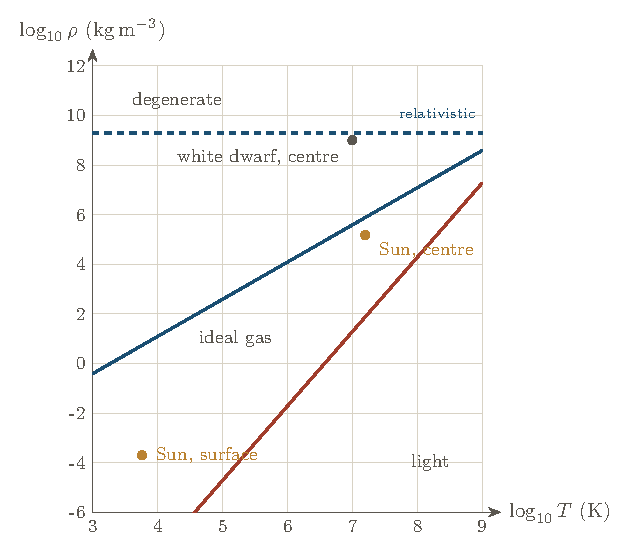
\includegraphics{fig_ch12_rho_T_plane.pdf}
	\caption{Density against temperature, on logarithmic axes. The red line marks equal pressure of light and of an ideal gas ($\mu=0.62$). The blue line marks a Fermi energy equal to $k_BT$ ($\mu_e=2$). The dashed line marks the density at which the electrons' Fermi momentum reaches $m_ec$. Points mark the centre and surface of the Sun and the centre of a white dwarf.}
	\label{st:fig:rho_T}
\end{figure}

The same counting gives the interiors of giant planets, the electron pressure of white dwarfs and neutron-star crusts, and, with nuclear physics, the burning in the Big Bang. It gives the composition, the degenerate pressure, the opacity and the burning rate.

\paragraph{Composition and mean molecular weight.} Let $X$, $Y$ and $Z$ be the mass fractions of hydrogen, helium and everything heavier, with $X+Y+Z=1$. In a fully ionised gas, a mass $m_{\rm H}$ of hydrogen gives two particles (a proton and an electron), a mass $4m_{\rm H}$ of helium gives three (a nucleus and two electrons), and a heavy atom of mass $Am_{\rm H}$ gives about $A/2$ particles (it has about $A/2$ electrons, and the one nucleus can be neglected). The number of particles per mass $m_{\rm H}$ is therefore
\begin{equation}
	\boxed{\frac{1}{\mu}=2X+\frac34Y+\frac12Z,\qquad \frac{1}{\mu_e}=X+\frac12Y+\frac12Z=\frac{1+X}{2},}
	\label{st:eq:mu}
\end{equation}
where $\mu$ is the mean molecular weight of Section~\ref{sg:sec:virial}, and $\mu_e$ counts the mass per electron, so that $n_e=\rho/(\mu_em_{\rm H})$. For the Sun's composition, $X=0.70$, $Y=0.28$, $Z=0.02$, this gives $\mu=0.617$ and $\mu_e=1.18$. Pure helium gives $\mu=\tfrac43$ and $\mu_e=2$, as do carbon and oxygen to good accuracy.

\paragraph{Degenerate electrons.} At high density and low temperature every electron state up to some momentum $p_F$, the \textbf{Fermi momentum}, is full and every state above it is empty. With two spin states, Eq.~\eqref{pr:eq:dn} gives the electron density
\begin{equation}
	n_e=\int_0^{p_F}\frac{2}{h^3}\,4\pi p^2\,dp=\frac{8\pi}{3h^3}\,p_F^3 ,\qquad p_F=h\left(\frac{3n_e}{8\pi}\right)^{1/3}.
	\label{st:eq:fermi}
\end{equation}
The pressure integral \eqref{pr:eq:pressure_integral} in the two limits of Section~\ref{pr:sec:p3} gives
\begin{align}
	P_{\rm slow}
	&\eqby{1} \frac13\int_0^{p_F}p\,\frac{p}{m_e}\,\frac{2}{h^3}4\pi p^2\,dp
	\eqby{2} \frac{8\pi p_F^5}{15\,m_eh^3}
	\eqby{3} \frac{h^2}{20\,m_e}\left(\frac3\pi\right)^{2/3}n_e^{5/3}, \nonumber\\
	P_{\rm fast}
	&\eqby{4} \frac13\int_0^{p_F}p\,c\,\frac{2}{h^3}4\pi p^2\,dp
	\eqby{5} \frac{2\pi c\,p_F^4}{3h^3}
	\eqby{6} \frac{hc}{8}\left(\frac3\pi\right)^{1/3}n_e^{4/3}.
	\label{st:eq:degenerate_P}
\end{align}
\begin{explain}
	\item Slow electrons, $v=p/m_e$.
	\item $\int_0^{p_F}p^4\,dp=p_F^5/5$.
	\item $p_F$ from Eq.~\eqref{st:eq:fermi}.
	\item Electrons at the speed of light, $v=c$.
	\item $\int_0^{p_F}p^3\,dp=p_F^4/4$.
	\item $p_F$ from Eq.~\eqref{st:eq:fermi}.
\end{explain}
With $n_e=\rho/(\mu_em_{\rm H})$ both are power laws of the density alone, $P\propto\rho^{5/3}$ for slow electrons and $P\propto\rho^{4/3}$ for fast ones, the two values of $\gamma$ from Eq.~\eqref{pr:eq:P_u}. The temperature does not appear. Heating degenerate gas does not raise its pressure, so it does not expand and cool, and the thermostat of Section~\ref{sg:sec:negheat} fails. Burning that starts in degenerate gas runs away, as in the helium flash of low-mass giants and in the thermonuclear explosion of a white dwarf. The ions stay classical, because at the same momentum their much larger mass gives them a far smaller kinetic energy.

\paragraph{When degeneracy matters.} Degeneracy matters when the Fermi energy $p_F^2/2m_e$ is comparable with $k_BT$, or equivalently when the spacing between electrons is comparable with their quantum wavelength (P6). Setting $p_F^2/2m_e=k_BT$ gives the blue line of Figure~\ref{st:fig:rho_T}, $\rho\propto T^{3/2}$. The electrons move near the speed of light when $p_F$ approaches $m_ec$, which by Eq.~\eqref{st:eq:fermi} with $\mu_e=2$ happens at $\rho=2.0\times10^9\,\mathrm{kg\,m^{-3}}$, the dashed line. The pressure of light exceeds that of the gas where $aT^4/3>\rho k_BT/(\mu m_{\rm H})$, below the red line, at low density and high temperature.

\paragraph{Opacity.} In hot, fully ionised gas the electrons scatter light with the Thomson cross-section, so $\kappa=\sigma_T/(\mu_em_{\rm H})=0.020(1+X)\,\mathrm{m^2\,kg^{-1}}$, independent of density and temperature. At lower temperatures, electrons bound to ions or passing close to them absorb light. Their cross-section falls with frequency roughly as $\nu^{-3}$, the light that carries the flux has $h\nu\sim k_BT$ (the Rosseland weighting of Section~\ref{rad:sec:diffusion}), and the number of absorbers per unit mass grows with the density. Together these give Kramers' law, $\kappa\propto\rho\,T^{-7/2}$, whose coefficient comes from atomic physics (the free–free part is derived in Eq.~\eqref{fp:eq:kramers}). Kramers opacity is what makes the outer layers of the Sun opaque enough to convect.

\paragraph{The burning rate and the Gamow peak.} Two protons at the Sun's centre, at $k_BT=1.35\,\mathrm{keV}$, approach each other against an electric barrier of about $1\,\mathrm{MeV}$. Classically they never touch. Quantum mechanically they tunnel, with a probability $e^{-\sqrt{E_G/E}}$ at relative energy $E$, where the \textbf{Gamow energy} $E_G=2m_rc^2(\pi\alpha Z_1Z_2)^2$ depends on their charges $Z_1,Z_2$ and their reduced mass $m_r$, and $\alpha$ is the fine-structure constant. For two protons, $E_G=493\,\mathrm{keV}$. The number of pairs at energy $E$ falls as the Maxwell tail $e^{-E/k_BT}$ (P3). The reaction rate is dominated by the energies where the product of the two is largest (Figure~\ref{st:fig:gamow}). Setting the derivative of its exponent to zero,
\begin{align}
	0
	&\eqby{1} \dv{E}\left(-\frac{E}{k_BT}-\sqrt{\frac{E_G}{E}}\right)
	\eqby{2} -\frac{1}{k_BT}+\frac12\,\frac{E_G^{1/2}}{E^{3/2}} \nonumber\\
	\implies\quad E_0
	&\eqby{3} \left(\frac{E_G\,(k_BT)^2}{4}\right)^{1/3}.
\end{align}
\begin{explain}
	\item The maximum of $e^{-E/k_BT}e^{-\sqrt{E_G/E}}$ is where its exponent is largest.
	\item $\dv*{}{E}\,E^{-1/2}=-\tfrac12E^{-3/2}$.
	\item Solve for $E$.
\end{explain}
\begin{equation}
	\boxed{E_0=\left(\frac{E_G\,(k_BT)^2}{4}\right)^{1/3}.}
	\label{st:eq:gamow}
\end{equation}
For the Sun's centre, $E_0=6.1\,\mathrm{keV}=4.5\,k_BT$. Only the rare protons far out on the Maxwell tail react, which is why a temperature of millions of kelvin, set by gravity through the virial theorem, is enough.

\begin{figure}[htbp]
	\centering
	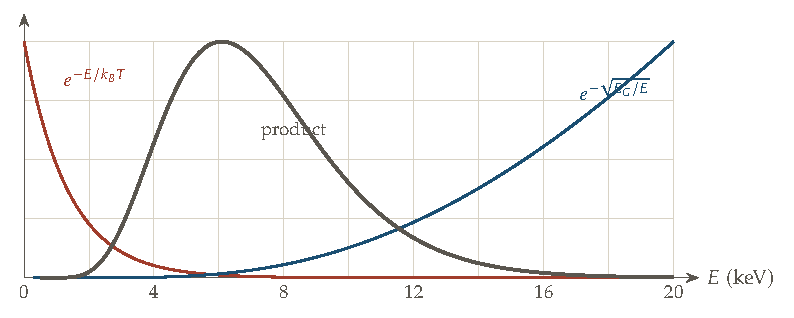
\includegraphics{fig_ch12_gamow.pdf}
	\caption{Two protons at the Sun's centre ($k_BT=1.35\,\mathrm{keV}$, $E_G=493\,\mathrm{keV}$). The Maxwell tail $e^{-E/k_BT}$, the tunnelling probability $e^{-\sqrt{E_G/E}}$, and their product, each scaled to a maximum of one within the range shown.}
	\label{st:fig:gamow}
\end{figure}

\paragraph{How steeply burning depends on temperature.} Near its peak the product is close to a Gaussian of width proportional to $(E_0k_BT)^{1/2}$, and its height is $e^{-3E_0/k_BT}$ (the two terms of the exponent at $E_0$ add to $3E_0/k_BT$). The rate per pair, averaged over the Maxwell distribution with its normalisation $(k_BT)^{-3/2}$, is therefore
\[
\text{rate}\propto(k_BT)^{-3/2}\,(E_0k_BT)^{1/2}\,e^{-3E_0/k_BT}\propto T^{-2/3}\,e^{-3E_0/k_BT},
\]
using $E_0\propto T^{2/3}$. Its logarithmic slope is
\begin{align}
	\dv{\ln(\text{rate})}{\ln T}
	&\eqby{1} -\frac23-\dv{\ln T}\left(\frac{3E_0}{k_BT}\right) \nonumber\\
	&\eqby{2} -\frac23+\frac{E_0}{k_BT} .
\end{align}
\begin{explain}
	\item The logarithm of the rate above.
	\item $3E_0/k_BT\propto T^{2/3}/T=T^{-1/3}$, so its logarithmic derivative is $-\tfrac13\times3E_0/k_BT$.
\end{explain}
For the proton–proton chain at the Sun's centre this is $3.8$, so its rate goes as about $T^4$. For the CNO cycle, whose slowest step is a proton meeting nitrogen ($Z_2=7$, $E_G=45\,\mathrm{MeV}$), it is about $20$. A one percent rise of temperature raises the CNO rate by twenty percent. This is why the thermostat of Section~\ref{sg:sec:negheat} holds the temperature of a burning core so tightly, why stars more massive than the Sun, whose hotter cores run on CNO, have convective cores, and why the temperature at which a fuel ignites is so sharply defined. Each fusion of four protons into helium releases $26.7\,\mathrm{MeV}$, $0.7\%$ of their rest mass, the figure used for the nuclear time in Section~\ref{sg:sec:freefall}.

% ==============================================================================
\section{Boundary Conditions and How Stars Are Computed}
\label{st:sec:computing}

The system \eqref{st:eq:system} has four unknowns and four first-order equations, now closed by the properties of the gas.

Four first-order equations need four conditions to fix a solution, and here they are split between the two ends. Two are known at the centre and two at the surface, and neither end alone fixes the star.

Think of building a bridge from both banks. Each team starts from its own bank with a guess for the height and slope of its half. The halves meet in the middle only if the guesses were right, and the gap between them says how to correct the guesses.

A star is computed the same way. Two conditions hold at the centre, two at the surface, and the solution must satisfy all four. Integrating from both ends and closing the gap in the middle, or adjusting the whole profile at once until every equation and every condition holds, gives the star. The method is conservation, applied numerically.

In numbers, a modern stellar model divides the star into about a thousand shells, so it solves for four thousand numbers at once, and repeats this for each of thousands of time steps over the star's life.

The picture is the bridge, two halves built toward each other until they meet.

The same two-ended problem appears in the interior of planets, in the structure of accretion disks and in many boundary-value problems of physics. It gives the boundary conditions, two ways to solve the system, and how a star is evolved in time.

\paragraph{Four boundary conditions.} At the centre there is no radius and no luminosity yet,
\begin{equation}
	r=0,\qquad L=0\qquad\text{at }m=0.
\end{equation}
At the surface the pressure has dropped to almost nothing and the temperature is that of the photosphere. With the grey atmosphere of Section~\ref{rad:sec:grey},
\begin{equation}
	P\approx0\ \ (\text{more exactly, the pressure at }\tau=\tfrac23),\qquad L=4\pi R^2\sigma_{\rm SB}T^4\qquad\text{at }m=M.
\end{equation}
The second surface condition says that the temperature at $m=M$ is the effective temperature. Two conditions at each end make this a \textbf{two-point boundary value problem}.

\paragraph{Shooting.} Guess the central pressure $P_c$ and temperature $T_c$ and integrate outward from the centre. Guess the radius $R$ and luminosity $L$ and integrate inward from the surface. Stop both at a fitting mass $m_f$ in between. The four differences between the two solutions there, $\Delta r$, $\Delta P$, $\Delta L$ and $\Delta T$, are functions of the four guesses. Newton's method corrects all four guesses at once,
\begin{equation}
	\begin{pmatrix}\delta P_c\\ \delta T_c\\ \delta R\\ \delta L\end{pmatrix}
	=-\left[\pdv{(\Delta r,\Delta P,\Delta L,\Delta T)}{(P_c,T_c,R,L)}\right]^{-1}
	\begin{pmatrix}\Delta r\\ \Delta P\\ \Delta L\\ \Delta T\end{pmatrix},
\end{equation}
where the $4\times4$ matrix of derivatives is found by repeating the integrations with each guess changed slightly. Near the centre the integration starts from the series $r\approx(3m/4\pi\rho_c)^{1/3}$, since the equations themselves are singular at $r=0$.

\paragraph{Relaxation.} Divide the star into $K$ shells and write the four unknowns at every shell boundary, $4K$ numbers in all. Replace each differential equation by its difference between neighbouring boundaries, $y_{k+1}-y_k=\Delta m\,f\big(\tfrac12(y_k+y_{k+1})\big)$ for the vector $y$ and right side $f$ of Eq.~\eqref{st:eq:system}. This gives $4(K-1)$ equations, and the four boundary conditions make $4K$. Starting from a guessed profile, Newton's method corrects all $4K$ numbers together. Each equation involves only two neighbouring shells, so the matrix of derivatives is zero except for small blocks along its diagonal, and it can be solved in a number of steps proportional to $K$. This is the Henyey method, used by modern codes such as MESA.

\paragraph{Evolution in time.} Burning changes the composition at each $m$, slowly, at rates set by $\varepsilon$. A star is evolved by alternating two steps. Advance the composition of every shell over a time step, then solve the four equations again for a new model in equilibrium. The ordering of the three clocks of Section~\ref{sg:sec:freefall} is what allows this, since the star regains hydrostatic equilibrium far faster than its composition changes. Given its mass and the composition at every $m$, the four equations with their boundary conditions fix the structure of a star. This is the Vogt–Russell statement, true for ordinary stars, though some sets of conditions admit more than one solution.

% ==============================================================================
\section{Polytropes and the Isothermal Sphere}
\label{st:sec:polytropes}

The full system \eqref{st:eq:system} needs a computer.

Insight often comes from a model simple enough to solve by hand, where the effect of each ingredient can be seen. Hydrostatic equilibrium and the mass equation alone involve only $P$, $\rho$ and $r$. They become solvable if the pressure depends on the density alone.

Think of a soft pillow and a firm one, each stacked with books. The firmness of the filling, how much its push grows when squeezed, decides how much the pillow flattens under a given weight. Nothing else about the pillow matters.

In a star the same is true when $P=\mathcal K\rho^\gamma$ for some constant $\mathcal K$. Then the stiffness $\gamma$ alone decides how the star's mass is spread out, and the mass equation with hydrostatic equilibrium (P1 and P2), closed by a pressure from counting states (P3), give one equation for the density. This happens for degenerate gas, where Eq.~\eqref{st:eq:degenerate_P} has exactly this form, and for gas that is convective throughout, where $P\propto\rho^\gamma$ along the adiabat.

In numbers, the model with $\gamma=\tfrac43$ scaled to the Sun's mass and radius gives a central density $\TwelveSunRhoC\,\mathrm{kg\,m^{-3}}$, a central pressure $\TwelveSunPC\,\mathrm{Pa}$ and a central temperature $\TwelveSunTC\,\mathrm K$, against $1.5\times10^5\,\mathrm{kg\,m^{-3}}$, $2.5\times10^{16}\,\mathrm{Pa}$ and $1.57\times10^7\,\mathrm K$ in detailed solar models.

The picture is Figure~\ref{st:fig:lane_emden}. A stiffer gas spreads the mass more evenly. A softer one concentrates it at the centre.

\begin{figure}[htbp]
	\centering
	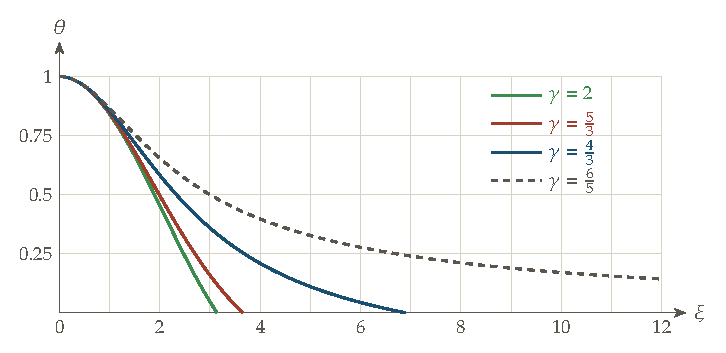
\includegraphics{fig_ch12_lane_emden.pdf}
	\caption{Solutions $\theta(\xi)$ of the Lane–Emden equation for $\gamma=2$, $\tfrac53$, $\tfrac43$ and $\tfrac65$. The density is $\rho_c\theta^{1/(\gamma-1)}$.}
	\label{st:fig:lane_emden}
\end{figure}

The same models describe white dwarfs and the cores of giant planets, fully convective low-mass stars, and, in the limit $\gamma\to1$, the isothermal sphere that models globular clusters and the dark matter halos of galaxies. They give one equation for the density, its solutions, the mass–radius relation, and two classic applications.

\paragraph{The Lane–Emden equation.} Divide hydrostatic equilibrium \eqref{sg:eq:hse} by $\rho$, multiply by $r^2$ and differentiate. With $\dv*{m}{r}=4\pi r^2\rho$,
\begin{equation}
	\frac{1}{r^2}\dv{r}\left(\frac{r^2}{\rho}\,\dv{P}{r}\right)=-4\pi G\rho .
	\label{st:eq:poisson_hse}
\end{equation}
Write the density as $\rho=\rho_c\,\theta^{1/(\gamma-1)}$, with $\rho_c$ the central density and $\theta=1$ at the centre. Then $P=\mathcal K\rho_c^\gamma\theta^{\gamma/(\gamma-1)}$, and
\begin{align}
	\frac1\rho\,\dv{P}{r}
	&\eqby{1} \frac{1}{\rho_c\theta^{1/(\gamma-1)}}\;\mathcal K\rho_c^\gamma\,\frac{\gamma}{\gamma-1}\,\theta^{1/(\gamma-1)}\,\dv{\theta}{r} \nonumber\\
	&= \frac{\gamma\,\mathcal K\rho_c^{\gamma-1}}{\gamma-1}\,\dv{\theta}{r} .
\end{align}
\begin{explain}
	\item The chain rule on $\theta^{\gamma/(\gamma-1)}$, whose exponent minus one is $1/(\gamma-1)$.
\end{explain}
Putting this into Eq.~\eqref{st:eq:poisson_hse} and measuring radius in the unit
\begin{equation}
	r_0^2=\frac{\gamma\,\mathcal K\,\rho_c^{\gamma-2}}{4\pi G(\gamma-1)},\qquad r=r_0\,\xi ,
	\label{st:eq:r0}
\end{equation}
all the constants collect into $r_0$ and
\begin{equation}
	\boxed{\frac{1}{\xi^2}\dv{\xi}\left(\xi^2\dv{\theta}{\xi}\right)=-\theta^{1/(\gamma-1)},\qquad\theta(0)=1,\quad\theta'(0)=0.}
	\label{st:eq:lane_emden}
\end{equation}
This is the \textbf{Lane–Emden equation}. The second condition says that the density is smooth at the centre. The surface of the star is the first zero $\xi_1$ of $\theta$, where density and pressure vanish.

\paragraph{Solutions.} Three values of $\gamma$ give solutions in closed form, which can be checked by putting them into Eq.~\eqref{st:eq:lane_emden}.
\begin{itemize}
	\item $\gamma\to\infty$, an incompressible star of uniform density, $\theta=1-\xi^2/6$, $\xi_1=\sqrt6$.
	\item $\gamma=2$, $\theta=\sin\xi/\xi$, $\xi_1=\pi$.
	\item $\gamma=\tfrac65$, $\theta=(1+\xi^2/3)^{-1/2}$, which never reaches zero. The radius is infinite, yet the mass is finite.
\end{itemize}
The two cases that matter most are solved numerically. For $\gamma=\tfrac53$, $\xi_1=\TwelveXiOneHalf$ and the central density is $\TwelveRhoRatioOneHalf$ times the mean density. For $\gamma=\tfrac43$, $\xi_1=\TwelveXiThree$ and the central density is $\TwelveRhoRatioThree$ times the mean.

\paragraph{Mass and radius.} The radius is $R=r_0\xi_1$. The mass follows from Eq.~\eqref{st:eq:lane_emden} itself,
\begin{align}
	M
	&\eqby{1} \int_0^R4\pi r^2\rho\,dr
	\eqby{2} 4\pi r_0^3\rho_c\int_0^{\xi_1}\xi^2\theta^{1/(\gamma-1)}\,d\xi \nonumber\\
	&\eqby{3} 4\pi r_0^3\rho_c\Big[-\xi^2\dv{\theta}{\xi}\Big]_{\xi_1}.
\end{align}
\begin{explain}
	\item The mass equation.
	\item $r=r_0\xi$ and $\rho=\rho_c\theta^{1/(\gamma-1)}$.
	\item Eq.~\eqref{st:eq:lane_emden} says $\xi^2\theta^{1/(\gamma-1)}=-\dv*{}{\xi}\big(\xi^2\dv*{\theta}{\xi}\big)$, and the term vanishes at $\xi=0$.
\end{explain}
For a fixed $\mathcal K$, Eq.~\eqref{st:eq:r0} gives $r_0\propto\rho_c^{(\gamma-2)/2}$, so $R\propto\rho_c^{(\gamma-2)/2}$ and $M\propto r_0^3\rho_c\propto\rho_c^{(3\gamma-4)/2}$. Eliminating $\rho_c$,
\begin{equation}
	\boxed{M\propto R^{(3\gamma-4)/(\gamma-2)}.}
	\label{st:eq:mass_radius}
\end{equation}
For $\gamma=\tfrac53$, $M\propto R^{-3}$. A heavier star of this kind is smaller, as white dwarfs are (Section~\ref{cs:sec:wd}). For $\gamma=\tfrac43$ the exponent vanishes. Only one mass is possible, whatever the radius. The factor $3\gamma-4$ is the one that made a star barely bound in Eq.~\eqref{sg:eq:E_gamma}.

\paragraph{The isothermal sphere.} As $\gamma\to1$ the gas has one temperature and $P=c_s^2\rho$. Writing $\rho=\rho_c e^{-\psi}$ and $r_0^2=c_s^2/(4\pi G\rho_c)$, Eq.~\eqref{st:eq:poisson_hse} becomes
\begin{equation}
	\frac{1}{\xi^2}\dv{\xi}\left(\xi^2\dv{\psi}{\xi}\right)=e^{-\psi},\qquad\psi(0)=0,\quad\psi'(0)=0 .
\end{equation}
The density never reaches zero, so an isothermal sphere has no surface. Far out it approaches a power law. Trying $\rho=A/r^2$ in hydrostatic equilibrium, with $m=4\pi Ar$,
\begin{align}
	c_s^2\,\dv{r}\left(\frac{A}{r^2}\right)
	&= -\frac{G\,(4\pi Ar)}{r^2}\,\frac{A}{r^2} \nonumber\\
	\implies\quad -\frac{2c_s^2A}{r^3}
	&= -\frac{4\pi GA^2}{r^3}
	\quad\implies\quad A=\frac{c_s^2}{2\pi G}.
\end{align}
So $\rho=c_s^2/(2\pi Gr^2)$, which is $\rho/\rho_c=2/\xi^2$. The numerical solution approaches this law (Figure~\ref{st:fig:isothermal}). At $\xi=10^4$ its density is $\TwelveIsoRatio$ of $2\rho_c/\xi^2$. The mass inside $r$ grows as $m=2c_s^2r/G$, so a body circling at radius $r$ has the speed
\begin{equation}
	v_{\rm circ}^2=\frac{Gm}{r}=2c_s^2,
\end{equation}
the same at every radius. Rotation curves of spiral galaxies are observed to be flat far beyond their visible stars. An isothermal halo of unseen matter is the simplest model that gives this, which is part of the case for dark matter.

\begin{figure}[htbp]
	\centering
	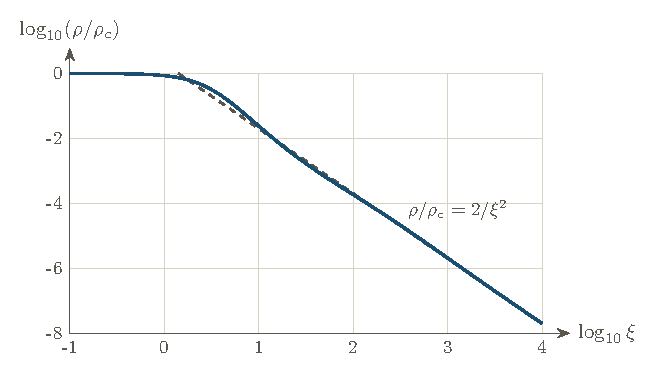
\includegraphics{fig_ch12_isothermal.pdf}
	\caption{The density of the isothermal sphere against radius, on logarithmic axes (solid), and the power law $\rho/\rho_c=2/\xi^2$ (dashed).}
	\label{st:fig:isothermal}
\end{figure}

\paragraph{Eddington's standard model, and the most massive stars.} Divide the momentum equation for light (Route B of Section~\ref{rad:sec:diffusion}, $\dv*{P_{\rm light}}{r}=-\kappa\rho L/(4\pi r^2c)$) by hydrostatic equilibrium \eqref{sg:eq:hse},
\begin{equation}
	\dv{P_{\rm light}}{P}=\frac{\kappa L(r)}{4\pi cG\,m(r)} .
\end{equation}
Eddington assumed that $\kappa L(r)/m(r)$ is about the same throughout the star. Then $P_{\rm light}$ is a fixed fraction of the total pressure everywhere. Call the gas fraction $\beta$, so $P_{\rm gas}=\beta P$ and $P_{\rm light}=(1-\beta)P$, with
\begin{equation}
	1-\beta=\frac{\kappa L}{4\pi cGM}=\frac{L}{L_{\rm Edd}},
	\label{st:eq:beta_edd}
\end{equation}
by Eq.~\eqref{rad:eq:eddington}. Eliminating $T$ between $P_{\rm gas}=\rho k_BT/(\mu m_{\rm H})$ and $P_{\rm light}=aT^4/3$,
\begin{align}
	T
	&\eqby{1} \frac{\mu m_{\rm H}\,\beta P}{k_B\rho} \nonumber\\
	\implies\quad (1-\beta)P
	&\eqby{2} \frac a3\left(\frac{\mu m_{\rm H}\,\beta P}{k_B\rho}\right)^4 \nonumber\\
	\implies\quad P
	&= \left[\frac{3(1-\beta)}{a\,\beta^4}\left(\frac{k_B}{\mu m_{\rm H}}\right)^4\right]^{1/3}\rho^{4/3} .
\end{align}
\begin{explain}
	\item The ideal-gas law for the gas share of the pressure.
	\item The pressure of light, Eq.~\eqref{pr:eq:photon_gas}.
\end{explain}
So the star is a polytrope with $\gamma=\tfrac43$, whose single mass is fixed by $\mathcal K$, and so by $\beta$. Turned around, the mass fixes $\beta$ through Eddington's quartic equation. The script gives $\beta=\TwelveBetaSun$ for the Sun, $\TwelveBetaTen$ at $10\,M_\odot$, $\TwelveBetaHundred$ at $100\,M_\odot$ and $\TwelveBetaThousand$ at $1000\,M_\odot$. In massive stars light carries a growing share of the pressure, Eq.~\eqref{st:eq:beta_edd} puts them close to the Eddington luminosity, and the effective $\gamma$ of their gas and light together falls toward $\tfrac43$, where Eq.~\eqref{sg:eq:E_gamma} leaves them barely bound. Stars much above about a hundred solar masses blow off their outer layers or become unstable, which sets the upper end of the masses of stars. The profiles of the solar model are drawn in Figure~\ref{st:fig:sun_profile}.

\begin{figure}[htbp]
	\centering
	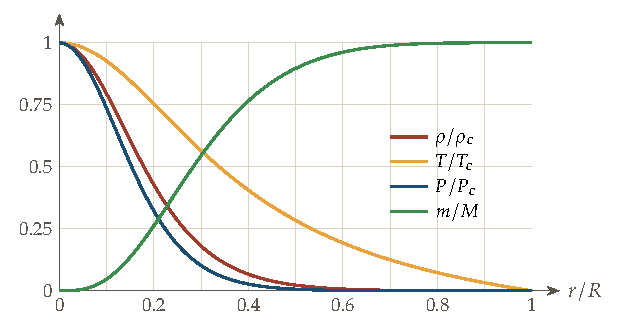
\includegraphics{fig_ch12_sun_profile.pdf}
	\caption{Eddington's standard model ($\gamma=\tfrac43$) scaled to the Sun. Density, temperature, pressure and enclosed mass against radius, each relative to its central or total value.}
	\label{st:fig:sun_profile}
\end{figure}

% ==============================================================================
\section{Scaling Laws and the HR Diagram}
\label{st:sec:scaling}

Polytropes gave the shape of a star. The full equations are needed for its luminosity.

Solving them for each mass is the work of a code. Yet the way luminosity and lifetime depend on mass can be read from the equations without solving them.

Think of model ships. A model built at half size, with everything in proportion, behaves in a way that can be predicted from the scale alone, without testing each new size from scratch.

Stars of different mass are close to scaled copies of each other. If every quantity in the four equations is replaced by its typical size, each equation becomes a relation between powers of $M$ and $R$. This is the comparison of scales (P6) applied to the equations themselves.

In numbers, the result $L\propto M^3$ for constant opacity, and the observed $L\propto M^{3.5}$ near the Sun, give a lifetime that falls as $M^{-2.5}$. A star of ten solar masses lives about $3\times10^7$ years, against $10^{10}$ for the Sun (Problem~\ref{st:prob:lifetimes}).

The picture is the HR diagram of Figure~\ref{st:fig:hr}, where stars of the same radius lie along straight lines.

\begin{figure}[htbp]
	\centering
	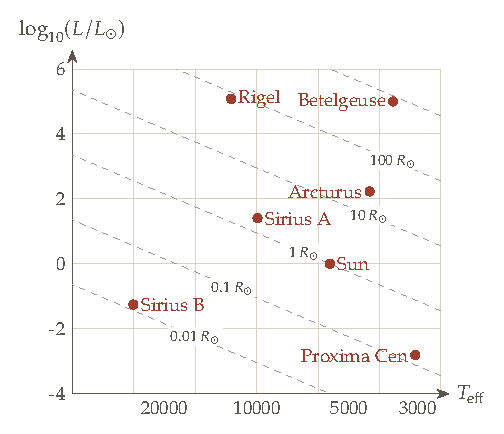
\includegraphics{fig_ch12_hr.pdf}
	\caption{Luminosity against effective temperature, with temperature increasing to the left, for $\TwelveHRN$ Hipparcos stars with parallaxes better than $10\%$ (all within $\TwelveHRMaxPc\,\mathrm{pc}$) and $\TwelveHRNwd$ Gaia white dwarfs within $100\,\mathrm{pc}$, coloured by temperature. Dashed lines join points of equal radius, labelled in solar radii. Circles mark seven well-known stars.}
	\label{st:fig:hr}
\end{figure}

The same scaling gives the relation between the speeds of stars in galaxies and the galaxies' luminosities, and the scaling relations of galaxy clusters. It gives the mass–luminosity relation, the smallest mass of a star, and the layout of the HR diagram.

\paragraph{Homology.} Replace $\dv*{}{m}$ by $1/M$, $r$ by $R$ and every other quantity by its typical size. The momentum equation \eqref{st:eq:momentum} and the ideal gas give
\begin{align}
	P
	&\sim \frac{GM^2}{R^4},\qquad
	T\sim\frac{\mu m_{\rm H}P}{k_B\rho}\sim\frac{\mu m_{\rm H}}{k_B}\,\frac{GM^2/R^4}{M/R^3}=\frac{\mu m_{\rm H}\,GM}{k_BR},
\end{align}
which is the virial temperature again. The radiative equation \eqref{st:eq:radiative} gives
\begin{align}
	L
	&\eqby{1} \frac{64\pi^2ac\,R^4T^4}{3\kappa M} \nonumber\\
	&\eqby{2} \frac{64\pi^2ac\,R^4}{3\kappa M}\left(\frac{\mu m_{\rm H}\,GM}{k_BR}\right)^4 \nonumber\\
	&\propto \frac{\mu^4M^3}{\kappa}.
\end{align}
\begin{explain}
	\item $\dv*{T}{m}\sim-T/M$ in Eq.~\eqref{st:eq:radiative}, solved for $L$.
	\item The temperature above.
\end{explain}
\begin{equation}
	\boxed{L\propto\frac{\mu^4M^3}{\kappa}.}
	\label{st:eq:mass_luminosity}
\end{equation}
The radius has dropped out, and so has the burning. A star's luminosity is set by how fast light can leak out of it, not by how fast it burns. The burning adjusts, through the thermostat, to supply what leaks out. With electron-scattering opacity, as in massive stars, $L\propto M^3$. Kramers opacity, which grows at the lower temperatures of smaller stars, steepens this, and near the Sun $L\propto M^{3.5}$ is observed. The fuel scales as $M$, so the lifetime scales as $M/L\propto M^{-2.5}$.

\paragraph{The smallest stars.} A contracting ball of gas heats up (Section~\ref{sg:sec:negheat}), but as its density rises its electrons become degenerate and start to push without heating. Add the electrons' Fermi energy to the virial balance of a uniform sphere of ionised hydrogen, with $N=M/m_{\rm H}$ protons and as many electrons. The protons carry the thermal energy, $\tfrac32Nk_B\bar T$, and the electrons their degenerate energy, $\tfrac35NE_F$ with $E_F=(\hbar^2/2m_e)(9\pi N/4R^3)^{2/3}$. The virial theorem, $2\times$ kinetic $=|U|=\tfrac35GM^2/R$, gives
\begin{equation}
	k_B\bar T=\frac{G M m_{\rm H}}{5R}-\frac{2}{5}E_F=\frac{\mathcal A}{R}-\frac{\mathcal B}{R^2},
\end{equation}
with $\mathcal A=GMm_{\rm H}/5$ and $\mathcal B=(\hbar^2/5m_e)(9\pi/4)^{2/3}N^{2/3}$. As $R$ shrinks the temperature first rises and then falls, with a maximum at $R=2\mathcal B/\mathcal A$,
\begin{equation}
	k_B\bar T_{\rm max}=\frac{\mathcal A^2}{4\mathcal B}\propto M^{4/3}.
\end{equation}
Hydrogen burns fast enough to stop the contraction only above a few million kelvin. Setting $\bar T_{\rm max}=3\times10^6\,\mathrm K$ gives $M\approx0.16\,M_\odot$. The centre of a star is about twice as hot as its mean, which lowers this to near the $0.08\,M_\odot$ found by detailed models. Lighter bodies never ignite hydrogen. They are brown dwarfs, and they cool forever at a radius near the peak, about $1.5$ times Jupiter's.

\paragraph{The HR diagram.} The Stefan–Boltzmann law, $L=4\pi R^2\sigma_{\rm SB}T_{\rm eff}^4$ (Eq.~\eqref{eq:stefan_boltzmann_luminosity}), gives
\[
\log L=2\log R+4\log T_{\rm eff}+\text{constant},
\]
so in a diagram of $\log L$ against $\log T_{\rm eff}$, stars of equal radius lie on straight lines (Figure~\ref{st:fig:hr}). Stars burning hydrogen in their cores form the main sequence, running from cool dim dwarfs like Proxima Centauri to hot bright stars like Sirius A, ordered by mass through Eq.~\eqref{st:eq:mass_luminosity}. Giants and supergiants like Arcturus and Betelgeuse lie above it at large radius, and white dwarfs like Sirius B below it at about a hundredth of the Sun's radius.

Each point in the figure is a real star. Its distance comes from its parallax (Section~\ref{as:sec:parallax}), and its brightness and distance give its luminosity. Its colour gives its temperature, and a small correction adds the light that falls outside the visual band. For the white dwarfs the catalogue gives the temperature, the surface gravity $g$ and the mass, so the radius is $R=\sqrt{GM/g}$ and the luminosity follows from Stefan–Boltzmann. The stars do not fill the diagram. Most sit on the main sequence, because a star spends about nine tenths of its life burning hydrogen in its core. The giant branch is thinner, since the giant stage is short. Hot bright stars are rare among the points, because massive stars are few and short-lived, and few lie within $\TwelveHRMaxPc\,\mathrm{pc}$. The dimmest red dwarfs, such as Proxima Centauri, were too faint for Hipparcos to measure well, so the main sequence stops above it in the figure.

A star leaves the main sequence when its core runs out of hydrogen. The core, now helium, has no burning to support it. It loses energy and, by Section~\ref{sg:sec:negheat}, contracts and heats. Hydrogen burns on in a shell around it, the shell's output rises as the core shrinks and heats, and the extra luminosity swells the envelope to a hundred times its former radius. The star moves to the upper right of the diagram and becomes a red giant. When the core reaches about $10^8\,\mathrm K$, helium ignites.

% ==============================================================================
\section{Problem Set: The Equations of a Star}

\subsection{Problem 1: Mean Molecular Weights}
\label{st:prob:mu}

\textbf{Problem Statement}: Find $\mu$ and $\mu_e$ for fully ionised gas of (a) solar composition, $X=0.70$, $Y=0.28$, $Z=0.02$, (b) pure helium, and (c) pure carbon.

\textbf{Essential Ideas}:
\begin{itemize}
	\item Count particles and electrons per mass $m_{\rm H}$, Eq.~\eqref{st:eq:mu}.
	\item Carbon, $A=12$, has a nucleus and six electrons, seven particles.
\end{itemize}

\textbf{Detailed Solutions}:
\begin{enumerate}[label=(\alph*)]
	\item \textbf{Solar}. $1/\mu=1.40+0.21+0.01=1.62$ and $1/\mu_e=0.85$.
	\[
	\boxed{\mu=0.62,\qquad\mu_e=1.18.}
	\]
	\item \textbf{Helium}. $1/\mu=\tfrac34$ and $1/\mu_e=\tfrac12$.
	\[
	\boxed{\mu=\tfrac43,\qquad\mu_e=2.}
	\]
	\item \textbf{Carbon}. Seven particles and six electrons per $12\,m_{\rm H}$.
	\[
	\boxed{\mu=\tfrac{12}{7}=1.71,\qquad\mu_e=2.}
	\]
\end{enumerate}

\subsection{Problem 2: Is It Degenerate?}
\label{st:prob:degeneracy}

\textbf{Problem Statement}: Compare the electrons' Fermi energy with $k_BT$ (a) at the Sun's centre ($\rho=1.5\times10^5\,\mathrm{kg\,m^{-3}}$, $T=1.57\times10^7\,\mathrm K$, $\mu_e=1.18$) and (b) at the centre of a white dwarf ($\rho=10^9\,\mathrm{kg\,m^{-3}}$, $T=10^7\,\mathrm K$, $\mu_e=2$). (c) In case (b), are the electrons relativistic?

\textbf{Essential Ideas}:
\begin{itemize}
	\item $n_e=\rho/(\mu_em_{\rm H})$, $p_F$ from Eq.~\eqref{st:eq:fermi}, $E_F=p_F^2/2m_e$ for slow electrons.
\end{itemize}

\textbf{Detailed Solutions}:
\begin{enumerate}[label=(\alph*)]
	\item \textbf{Sun}.
	\[
	\boxed{E_F/k_BT\simeq0.5.}
	\]
	Mildly degenerate. The ideal-gas law is accurate to some percent there.
	\item \textbf{White dwarf}.
	\[
	\boxed{E_F/k_BT\simeq190.}
	\]
	Strongly degenerate. The temperature barely matters for the pressure.
	\item \textbf{Relativistic?} $p_F/m_ec=0.80$. The electrons move at a large fraction of $c$, and neither limit of Eq.~\eqref{st:eq:degenerate_P} is exact.
\end{enumerate}

\subsection{Problem 3: The Gamow Peak}
\label{st:prob:gamow}

\textbf{Problem Statement}: At the Sun's centre, $k_BT=1.35\,\mathrm{keV}$. (a) Find the Gamow peak $E_0$ for two protons ($E_G=493\,\mathrm{keV}$) and the temperature exponent of the rate. (b) Repeat for a proton and a nitrogen nucleus ($E_G=45\,\mathrm{MeV}$).

\textbf{Essential Ideas}:
\begin{itemize}
	\item $E_0=(E_G(k_BT)^2/4)^{1/3}$, Eq.~\eqref{st:eq:gamow}, and the exponent $E_0/k_BT-\tfrac23$.
\end{itemize}

\textbf{Detailed Solutions}:
\begin{enumerate}[label=(\alph*)]
	\item \textbf{Two protons}. $E_0=(493\times1.35^2/4)^{1/3}\,\mathrm{keV}$.
	\[
	\boxed{E_0\simeq6.1\,\mathrm{keV}=4.5\,k_BT,\qquad\text{rate}\propto T^{3.8}.}
	\]
	\item \textbf{Proton and nitrogen}.
	\[
	\boxed{E_0\simeq27\,\mathrm{keV}=20\,k_BT,\qquad\text{rate}\propto T^{19.6}.}
	\]
\end{enumerate}

\subsection{Problem 4: Lifetimes}
\label{st:prob:lifetimes}

\textbf{Problem Statement}: Take $L\propto M^{3.5}$ and a main-sequence lifetime of $10^{10}$ years for the Sun. Estimate the lifetimes of stars of $0.5$, $10$ and $50\,M_\odot$.

\textbf{Essential Ideas}:
\begin{itemize}
	\item Lifetime $\propto M/L\propto M^{-2.5}$.
\end{itemize}

\textbf{Detailed Solutions}:
\[
\boxed{0.5\,M_\odot:\ 6\times10^{10}\ \text{yr},\qquad 10\,M_\odot:\ 3\times10^{7}\ \text{yr},\qquad 50\,M_\odot:\ 6\times10^{5}\ \text{yr}.}
\]
Every star of half a solar mass ever formed is still on the main sequence, since the universe is only $1.4\times10^{10}$ years old. Massive stars live and die while the cloud they formed in is still nearby.

\subsection{Problem 5: The Temperature Fall of the Earth's Air}
\label{st:prob:lapse}

\textbf{Problem Statement}: The Earth's lower atmosphere is stirred by convection. Use the convective gradient, Eq.~\eqref{st:eq:convective}, with $\gamma=\tfrac75$ for air (mean molecular mass $28.97\,\mathrm u$) and hydrostatic equilibrium near the ground to find how fast the temperature falls with height.

\textbf{Essential Ideas}:
\begin{itemize}
	\item $\dv*{\ln T}{\ln P}=(\gamma-1)/\gamma$, and $\dv*{P}{z}=-\rho g$ with $\rho=P\mu m_{\rm H}/(k_BT)$.
\end{itemize}

\textbf{Detailed Solutions}:
\begin{align*}
	\dv{T}{z}
	&\eqby{1} \frac{T}{P}\,\frac{\gamma-1}{\gamma}\,\dv{P}{z}
	\eqby{2} -\frac{\gamma-1}{\gamma}\,\frac{\mu m_{\rm H}\,g}{k_B}.
\end{align*}
\begin{explain}
	\item The convective gradient.
	\item Hydrostatic equilibrium with the ideal gas, $\dv*{P}{z}=-P\mu m_{\rm H}g/(k_BT)$.
\end{explain}
\[
\boxed{\dv{T}{z}=-\frac27\times\frac{28.97\times1.661\times10^{-27}\times9.81}{1.381\times10^{-23}}\,\mathrm{K\,m^{-1}}\simeq-9.8\,\mathrm{K\,km^{-1}}.}
\]
This is the dry adiabatic lapse rate of meteorology. The same criterion that decides where the Sun convects decides how cold mountain tops are.
